\label{sec:anatomical-scale-preference}
The retained granularities favor different anatomical regions. We compare ZoomST Spatial representations at granularities 8, 32, and 128 with six external methods across all 43 regions in the eight held-out sections. For each section, all methods share annotation-balanced clustering-fit positions and are scored on the full section by region-wise IoU (Appendix~\ref{app:region-scale}). Table~\ref{tab:regional-spatial-iou} highlights two patterns from the complete benchmark in Table~\ref{tab:regional-spatial-iou-full}. Locally homogeneous Spinal cord, Kidney, and Olfactory epithelium favor granularity 128, whereas boundary-rich Mucosal epithelium, Blood vessel, and Surface ectoderm favor granularity 8. Spinal cord IoU rises from 0.390 at granularity 8 to 0.489 at 128, while Blood vessel falls from 0.347 to 0.138. In these examples, the preferred ZoomST granularity also exceeds all six external methods. The choice of context therefore changes which anatomical structures the representation resolves best.

These scale preferences track the composition of the surrounding tissue. We measure neighborhood homogeneity by the mean same-label fraction among 128 spatial neighbors, and boundary fraction by the proportion of positions with at least one differently labeled neighbor among their eight nearest neighbors. Across 137 section--region observations, the coarse-scale gain, $\Delta\mathrm{IoU}=\mathrm{IoU}_{128}-\mathrm{IoU}_{8}$, increases with homogeneity and decreases with boundary fraction (Figure~\ref{fig:region-geometry}). The mean within-section Spearman correlations are 0.409 and $-0.337$, respectively, with each direction observed in seven of eight sections. Locally homogeneous structures therefore tend to benefit more from broad context, while regions with frequent boundaries favor finer context. The representations thus retain distinct anatomical uses after cross-granularity learning.

\begin{figure}[!htbp]
\centering
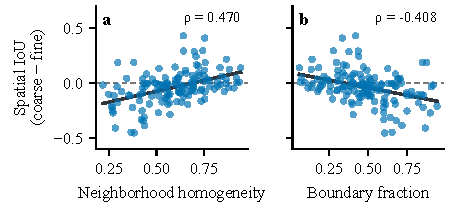
\includegraphics[width=\linewidth]{figures/region_geometry.pdf}
\caption{\textbf{Coarse-scale anatomical gains track neighborhood homogeneity and boundary frequency.} Each point is one of 137 section--region observations from eight held-out sections; colors and symbols identify developmental stages. The vertical axis is the Spatial IoU difference between granularities 128 and 8, in percentage points, after averaging three clustering seeds. Positive values favor coarse context. (a) Mean same-label fraction among 128 spatial neighbors. (b) Fraction of positions with a differently labeled neighbor among eight spatial neighbors. Geometry uses the full measured section, excluding each focal position from its own neighbor set. Solid lines show pooled linear fits; dashed lines mark equal IoU. The panels report pooled Spearman correlations and the mean of eight within-section correlations.}
\label{fig:region-geometry}
\end{figure}
\FloatBarrier
\begin{table}[!htbp]
\begingroup\centering\fontsize{8}{9}\selectfont
\setlength{\tabcolsep}{1.1pt}\renewcommand{\arraystretch}{1.02}
\caption{\textbf{Distinct anatomical structures favor coarse or fine Spatial context.} Selected examples from the complete 43-region benchmark in Table~\ref{tab:regional-spatial-iou-full}. The upper group favors granularity 128; the lower group favors granularity 8. In each example, the preferred ZoomST granularity also attains the highest IoU among the compared methods. Values are means with sample SD below across $n$ sections, after averaging three clustering seeds per section; single-section regions have one value. $H_{128}$ is neighborhood homogeneity. Bold marks the highest IoU across columns; underlining marks the best ZoomST granularity.}\label{tab:regional-spatial-iou}
\begin{tabular}{@{}>{\raggedright\arraybackslash}p{0.175\linewidth}cc*{9}{c}@{}}
\toprule
 & & & \multicolumn{3}{c}{ZoomST Spatial} & \multicolumn{2}{c}{Frozen pretrained} & \multicolumn{4}{c}{Target-fitted} \\
\cmidrule(lr){4-6}\cmidrule(lr){7-8}\cmidrule(l){9-12}
Region & $n$ & $H_{128}$ & 8 & 32 & 128 & Novae & SToFM & GraphST & BANKSY & MENDER & STAGATE \\
\midrule
\multicolumn{12}{l}{\textit{Coarse-context examples}}\\[3pt]
Spinal cord & 4 & 0.780 & \shortstack{0.390\\{\fontsize{7}{7.5}\selectfont $\pm0.108$}} & \shortstack{0.404\\{\fontsize{7}{7.5}\selectfont $\pm0.065$}} & \shortstack{\textbf{\underline{0.489}}\\{\fontsize{7}{7.5}\selectfont $\pm0.117$}} & \shortstack{0.311\\{\fontsize{7}{7.5}\selectfont $\pm0.172$}} & \shortstack{0.198\\{\fontsize{7}{7.5}\selectfont $\pm0.082$}} & \shortstack{0.436\\{\fontsize{7}{7.5}\selectfont $\pm0.166$}} & \shortstack{0.398\\{\fontsize{7}{7.5}\selectfont $\pm0.119$}} & \shortstack{0.402\\{\fontsize{7}{7.5}\selectfont $\pm0.089$}} & \shortstack{0.426\\{\fontsize{7}{7.5}\selectfont $\pm0.154$}} \\[2.2pt]
Kidney & 1 & 0.755 & 0.286 & 0.425 & \textbf{\underline{0.697}} & 0.045 & 0.136 & 0.639 & 0.007 & 0.007 & 0.112 \\[2.2pt]
Olfactory epithelium & 2 & 0.750 & \shortstack{0.540\\{\fontsize{7}{7.5}\selectfont $\pm0.372$}} & \shortstack{0.572\\{\fontsize{7}{7.5}\selectfont $\pm0.196$}} & \shortstack{\textbf{\underline{0.616}}\\{\fontsize{7}{7.5}\selectfont $\pm0.061$}} & \shortstack{0.412\\{\fontsize{7}{7.5}\selectfont $\pm0.027$}} & \shortstack{0.040\\{\fontsize{7}{7.5}\selectfont $\pm0.020$}} & \shortstack{0.528\\{\fontsize{7}{7.5}\selectfont $\pm0.301$}} & \shortstack{0.552\\{\fontsize{7}{7.5}\selectfont $\pm0.299$}} & \shortstack{0.463\\{\fontsize{7}{7.5}\selectfont $\pm0.433$}} & \shortstack{0.194\\{\fontsize{7}{7.5}\selectfont $\pm0.266$}} \\[2.2pt]
\midrule
\multicolumn{12}{l}{\textit{Fine-context examples}}\\[3pt]
Mucosal epithelium & 4 & 0.518 & \shortstack{\textbf{\underline{0.302}}\\{\fontsize{7}{7.5}\selectfont $\pm0.178$}} & \shortstack{0.260\\{\fontsize{7}{7.5}\selectfont $\pm0.112$}} & \shortstack{0.188\\{\fontsize{7}{7.5}\selectfont $\pm0.122$}} & \shortstack{0.221\\{\fontsize{7}{7.5}\selectfont $\pm0.174$}} & \shortstack{0.076\\{\fontsize{7}{7.5}\selectfont $\pm0.022$}} & \shortstack{0.270\\{\fontsize{7}{7.5}\selectfont $\pm0.189$}} & \shortstack{0.196\\{\fontsize{7}{7.5}\selectfont $\pm0.153$}} & \shortstack{0.212\\{\fontsize{7}{7.5}\selectfont $\pm0.160$}} & \shortstack{0.290\\{\fontsize{7}{7.5}\selectfont $\pm0.242$}} \\[2.2pt]
Blood vessel & 2 & 0.439 & \shortstack{\textbf{\underline{0.347}}\\{\fontsize{7}{7.5}\selectfont $\pm0.254$}} & \shortstack{0.306\\{\fontsize{7}{7.5}\selectfont $\pm0.110$}} & \shortstack{0.138\\{\fontsize{7}{7.5}\selectfont $\pm0.193$}} & \shortstack{0.127\\{\fontsize{7}{7.5}\selectfont $\pm0.039$}} & \shortstack{0.182\\{\fontsize{7}{7.5}\selectfont $\pm0.227$}} & \shortstack{0.001\\{\fontsize{7}{7.5}\selectfont $\pm0.001$}} & \shortstack{0.134\\{\fontsize{7}{7.5}\selectfont $\pm0.153$}} & \shortstack{0.218\\{\fontsize{7}{7.5}\selectfont $\pm0.231$}} & \shortstack{0.296\\{\fontsize{7}{7.5}\selectfont $\pm0.307$}} \\[2.2pt]
Surface ectoderm & 2 & 0.428 & \shortstack{\textbf{\underline{0.399}}\\{\fontsize{7}{7.5}\selectfont $\pm0.059$}} & \shortstack{0.304\\{\fontsize{7}{7.5}\selectfont $\pm0.063$}} & \shortstack{0.312\\{\fontsize{7}{7.5}\selectfont $\pm0.029$}} & \shortstack{0.154\\{\fontsize{7}{7.5}\selectfont $\pm0.054$}} & \shortstack{0.174\\{\fontsize{7}{7.5}\selectfont $\pm0.016$}} & \shortstack{0.256\\{\fontsize{7}{7.5}\selectfont $\pm0.133$}} & \shortstack{0.301\\{\fontsize{7}{7.5}\selectfont $\pm0.051$}} & \shortstack{0.226\\{\fontsize{7}{7.5}\selectfont $\pm0.157$}} & \shortstack{0.342\\{\fontsize{7}{7.5}\selectfont $\pm0.068$}} \\[2.2pt]
\bottomrule
\end{tabular}\par\endgroup
\end{table}

